\documentclass{beamer}

\usepackage[utf8]{inputenc}


\usepackage{tikz,amsmath, amssymb,bm,color}
\usetikzlibrary{overlay-beamer-styles}

\tikzstyle{normal}=[circle,fill=white, draw=black, thick]

\usetheme{Boadilla}

%Information to be included in the title page:
\title[Graph Algorithms with Hostile Partners]{Introduction to Graph Algorithms with Hostile Partners}
\author{Matthew Askes}
\institute[Victoria University]{Victoria University of Wellington}
\date{2020}



\begin{document}

\frame{\titlepage}

\begin{frame}
    \frametitle{The Dinner Party Problem}
    Alice is hosting a dinner party. The guests are lazy and hungry.     
    
    \bigskip
    \pause
    
    If a guest receives a platter they distribute food to their immediate neighbours.
    
    \bigskip
    \pause
    
    Alice attempts to minimise the number of platters.
    
\end{frame}

\begin{frame}% # 00
    \frametitle{A Graph of the Party}
    
    \begin{block}{Defination}        
        A Graph $G$ is a pair $(V,E)$, where $V$ is a set of elements called vertices and $E$ a set of pairs of vertices called edges. 
    \end{block}
    
\end{frame}


\begin{frame}
    \frametitle{A Minimum Number of Platters}    
    \begin{figure}
        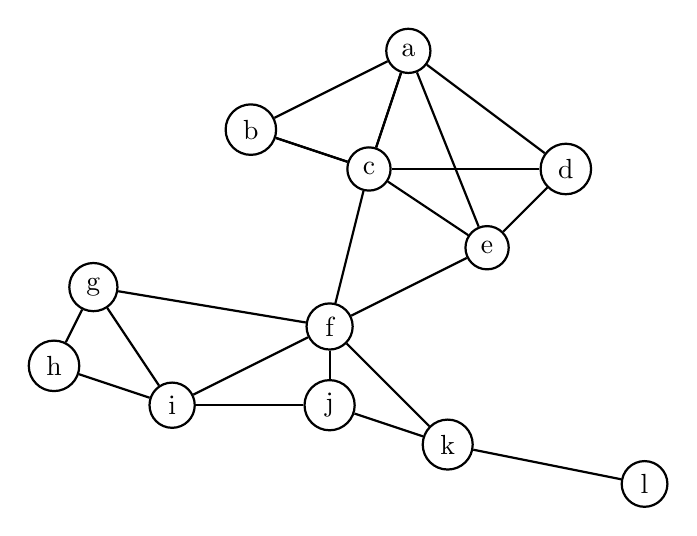
\begin{tikzpicture}
        
        \node [normal] (v11) at (-2.5,4) {a};
        \node [normal] (v9) at (-4.5,3) {b};
        \node [normal, alt=<2>{fill=red}{fill=white}] (v10) at (-3,2.5) {c};
        \node [normal] (v12) at (-0.5,2.5) {d};
        \node [normal] (v8) at (-1.5,1.5) {e};
        \node [normal] (v4) at (-3.5,0.5) {f};
        \node [normal] (v3) at (-6.5,1) {g};
        \node [normal, alt=<2>{fill=red}{fill=white}] (v1) at (-7,0) {h};
        \node [normal] (v2) at (-5.5,-0.5) {i};
        \node [normal] (v5) at (-3.5,-0.5) {j};
        \node [normal, alt=<2>{fill=red}{fill=white}] (v6) at (-2,-1) {k};
        \node [normal] (v7) at (0.5,-1.5) {l};
        \draw [thick] (v1) edge (v2);
        \draw [thick] (v3) edge (v2);
        \draw [thick] (v1) edge (v3);
        \draw [thick] (v4) edge (v5);
        \draw [thick] (v6) edge (v5);
        \draw [thick] (v6) edge (v7);
        \draw [thick] (v8) edge (v4);
        \draw [thick] (v2) edge (v4);
        \draw [thick] (v4) edge (v3);
        \draw [thick] (v2) edge (v5);
        \draw [thick] (v4) edge (v6);
        \draw [thick] (v9) edge (v10);
        \draw [thick] (v10) edge (v11);
        \draw [thick] (v9) edge (v10);
        \draw [thick] (v8) edge (v12);
        \draw [thick] (v10) edge (v11);
        \draw [thick] (v12) edge (v10);
        \draw [thick] (v4) edge (v10);
        \draw [thick] (v9) edge (v11);
        \draw [thick] (v11) edge (v8);
        \draw [thick] (v11) edge (v12);
        \draw [thick] (v10) edge (v8);
        \end{tikzpicture}
        \caption{The graph of the party}
    \end{figure}
    \uncover<2->{
    A dominating set is $\{c,h,k\}$
    }
\end{frame}


\begin{frame}
    \frametitle{Dominating sets}
    
    \begin{block}{Defination}        
        A dominating set, $D$, is a set of vertices such that vertex in $V(G)$ is a adjacent to at least one vertex in $D$.
    \end{block}
    
\end{frame}

\begin{frame}
    \frametitle{The Dinner Party Problem}
    Alice hosts another dinner party. The guests are lazy and hungry.     
    
    \bigskip
    \pause
    
    If a guest receives a platter they distribute food to their nearest guests.
    
    \bigskip
    \pause
    
    Alternating Alice and Bob hand out platters.
    
    \bigskip
    \pause
    
    Alice attempts to minimise the number of platters. 
    
    \bigskip
    \pause
    
    Bob is a hostile partner.
\end{frame}

\begin{frame}
    \frametitle{Not enough Platters}    
    \begin{figure}
        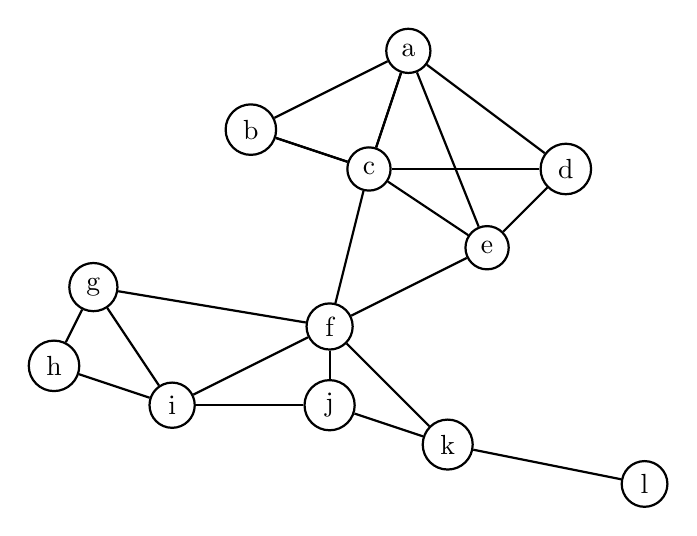
\begin{tikzpicture}
        
        
        \node [normal] (v11) at (-2.5,4) {a};
        \node [normal] (v9) at (-4.5,3) {b};
        \node [normal, alt=<4->{fill=red}{fill=white}] (v10) at (-3,2.5) {c};
        \node [normal] (v12) at (-0.5,2.5) {d};
        \node [normal] (v8) at (-1.5,1.5) {e};
        \node [normal] (v4) at (-3.5,0.5) {f};
        \node [normal, alt=<5>{draw=red}{draw=black}] (v3) at (-6.5,1) {g};
        \node [normal, alt=<5>{draw=red}{draw=black}] (v1) at (-7,0) {h};
        \node [normal] (v2) at (-5.5,-0.5) {i};
        \node [normal, alt=<3->{fill=blue}{fill=white}] (v5) at (-3.5,-0.5) {j};
        \node [normal, alt=<2->{fill=red}{fill=white}] (v6) at (-2,-1) {k};
        \node [normal] (v7) at (0.5,-1.5) {l};
        \draw [thick] (v1) edge (v2);
        \draw [thick] (v3) edge (v2);
        \draw [thick] (v1) edge (v3);
        \draw [thick] (v4) edge (v5);
        \draw [thick] (v6) edge (v5);
        \draw [thick] (v6) edge (v7);
        \draw [thick] (v8) edge (v4);
        \draw [thick] (v2) edge (v4);
        \draw [thick] (v4) edge (v3);
        \draw [thick] (v2) edge (v5);
        \draw [thick] (v4) edge (v6);
        \draw [thick] (v9) edge (v10);
        \draw [thick] (v10) edge (v11);
        \draw [thick] (v9) edge (v10);
        \draw [thick] (v8) edge (v12);
        \draw [thick] (v10) edge (v11);
        \draw [thick] (v12) edge (v10);
        \draw [thick] (v4) edge (v10);
        \draw [thick] (v9) edge (v11);
        \draw [thick] (v11) edge (v8);
        \draw [thick] (v11) edge (v12);
        \draw [thick] (v10) edge (v8);
        \end{tikzpicture}
        \caption{The graph of the party}
    \end{figure}

\end{frame}
\begin{frame}
    \frametitle{The Dinner Party Problem}
    What is the smallest number of platters that Alice needs to ensure everyone is feed?
    
    \bigskip
    \pause
    
    For our party it is 5.
    
\end{frame}

\begin{frame}
    \frametitle{An Optimal Number of Platters}    
    \begin{figure}
        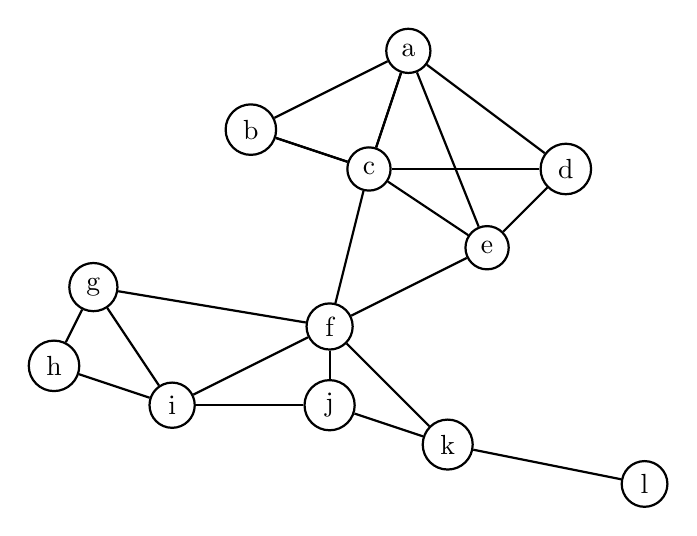
\begin{tikzpicture}
        
        \node [normal] (v11) at (-2.5,4) {a};
        \node [normal] (v9) at (-4.5,3) {b};
        \node [normal, alt=<4->{fill=red}{fill=white}] (v10) at (-3,2.5) {c};
        \node [normal] (v12) at (-0.5,2.5) {d};
        \node [normal] (v8) at (-1.5,1.5) {e};
        \node [normal, alt=<5->{fill=blue}{fill=white}] (v4) at (-3.5,0.5) {f};
        \node [normal] (v3) at (-6.5,1) {g};
        \node [normal, alt=<6->{fill=red}{fill=white}] (v1) at (-7,0) {h};
        \node [normal] (v2) at (-5.5,-0.5) {i};
        \node [normal, alt=<3->{fill=blue}{fill=white}] (v5) at (-3.5,-0.5) {j};
        \node [normal, alt=<2->{fill=red}{fill=white}] (v6) at (-2,-1) {k};
        \node [normal] (v7) at (0.5,-1.5) {l};
        
        \draw [thick] (v1) edge (v2);
        \draw [thick] (v3) edge (v2);
        \draw [thick] (v1) edge (v3);
        \draw [thick] (v4) edge (v5);
        \draw [thick] (v6) edge (v5);
        \draw [thick] (v6) edge (v7);
        \draw [thick] (v8) edge (v4);
        \draw [thick] (v2) edge (v4);
        \draw [thick] (v4) edge (v3);
        \draw [thick] (v2) edge (v5);
        \draw [thick] (v4) edge (v6);
        \draw [thick] (v9) edge (v10);
        \draw [thick] (v10) edge (v11);
        \draw [thick] (v9) edge (v10);
        \draw [thick] (v8) edge (v12);
        \draw [thick] (v10) edge (v11);
        \draw [thick] (v12) edge (v10);
        \draw [thick] (v4) edge (v10);
        \draw [thick] (v9) edge (v11);
        \draw [thick] (v11) edge (v8);
        \draw [thick] (v11) edge (v12);
        \draw [thick] (v10) edge (v8);
        \end{tikzpicture}
        \caption{The graph of the party}
    \end{figure}
\end{frame}

\begin{frame}
    \frametitle{Game Domination Number}
    
    \begin{block}{Defination}        
      For a graph $G$ the game domination number of $G$, is the size of the smallest dominating set in $G$ that Alice can guarantee exists with Bob as a hostile partner. 
    \end{block}
    
    \bigskip
    \pause
    
    What is the game domination number for a general graph? 
    
\end{frame}

\begin{frame}
\frametitle{Any questions?}

Thank you for your attention.


\vfill
An implementation of the colouring game is available at the following link.

bit.ly/GraphColouringGame

\end{frame}



\end{document}